
\chapter{Caso Práctico: Selección de Estructura de Datos}
\label{data_struct_sel}

A esta altura ya aprendiste sobre las estructuras de datos principales
de Perl, y has visto algunos de los algoritmos que las usan.

Este capítulo presenta un caso práctico con ejercicios que te dejan 
pensar acerca de la elección de estructuras de datos y practicar 
usándolas.

Pero primero, me gustaría discutir brevemente dos estructuras condicionales
que hemos ignorado hasta ahora y proveer nuevas posibilidades sobre las
signaturas de una subrutina.
\index{signature}

\section{El Operador Condicional Ternario}
\label{ternary operator}
\index{ternary conditional operator}

Considera el siguiente código que verifica el valor de un
número entero positivo:

\begin{verbatim}
my $result;
if $num < 10 {
    $result = "Un dígito";
} else {
    $result = "Más de un dígito";
}
say $result;
\end{verbatim}

Esto es bien simple, pero un poco largo. Esto puede escribirse
en una sola línea de código en la siguiente forma:

\begin{verbatim}
say $num < 10 ?? "Un dígito" !! "Más de un dígito";
\end{verbatim}

El operador está conformado por dos partes: {\tt ??} y {\tt !!},
los cuales separan tres expresiones (de ahí su nombre de ``operador ternario``):
\index{ternary operator}
\index{operator!ternary}
\begin{itemize}
\item La condición a ser evaluada (?`es \verb|$num| menor que 10?);
\item La expresión que define el valor si la condición es verdadera;
\item La expresión que define el valor si la condición es falsa.
\end{itemize}

Esta sentencia chequea si \verb|$num| es menor que 10 y, si esto es verdadero,
imprime ``Un dígito``; si la condición es falsa, entonces imprime ``Más de un dígito``.

Este operador no provee una funcionalidad nueva; solo ofrece una sintaxis
más concisa.

Es posible anidar varios operadores ternarios para examinar múltiples opciones
sucesivamente:
\index{ternary conditional operator, nesting}

\begin{verbatim}
say $valor < 10    ?? "Un dígito"     !! 
    $valor < 100   ?? "Dos dígitos"   !!
    $valor < 1000  ?? "Tres dígitos"  !!
                      "Más de tres dígitos";
\end{verbatim}

Esta construcción es una forma de sentencia conocida algunas
veces como una \emph{sentencia de switch} porque el lenguaje
C y muchos lenguajes derivados del mismo usan la palabra clave
{\tt switch} para describir una condicional con opciones múltiples.
\index{switch statement}

Esto es mucho más conciso y usualmente más conveniente que las condicionales
anidadas {\tt if ... después ... else}, pero la siguiente sección provee un
tipo de sentencia {\tt switch} mucho más poderosa.

\section{La Sentencia ``Switch'' {\tt given ... when}}
\label{given_when}
\index{given statement}
\index{when statement}
\index{switch statement}

Perl~6 tiene una sentencia ``switch'', escrita con las palabras claves 
{\tt given} y {\tt when}. La palabra clave {\tt given} introduce la variable
o expresión que será puesta a prueba, y cada una de las sentencia {\tt when}
especifica una condición seguida por un bloque que se ejecutará si la 
condición es verdadera. Por defecto, el proceso para cuando la primera
con la primera condición que es satisfecha.

El ejemplo más arriba podría escribirse como sigue:

\begin{verbatim}
given $value {
    when 0..9      { say "Un dígito" }
    when $_ < 99   { say "Dos dígitos" }
    when /^\d**3$/ { say "Tres dígitos" }
    default        { say "Más de tres dígitos" }
}
\end{verbatim}

La sentencia \verb|given $valor| ``topicaliza`` el argumento, i.e., 
asigna el contexto de \verb|$valor| a la variable tópico \verb|$_|
(o, más precisamente, crea un sobrenombre del mismo a través de 
la variable \verb|$_|). El argumento de {\tt given} es una variable simple
en el ejemplo más arriba, pero puede ser una expresión compleja cuya evaluación
se almacena en \verb|$_|. Cada una de las condiciones {\tt when} es
chequeada contra \verb|$_|. He escrito estas condiciones en tres formas
sintácticas diferentes para ilustrar algunas de las varias posibilidades:
\index{topical variable}
\index{alias}
\begin{itemize}
\item La primera chequea contra \verb|$_| (implícitamente) contra el
rango \verb|0..9|.
\index{range operator}
\item La segunda compara explícitamente \verb|$_| con 99.
\item La tercera usa un regex para chequear si \verb|$_| tiene
tres dígitos.
\index{regex}
\item La sentencia \verb|default| se ejecuta solo si las otras condiciones
han fallado.
\index{default statement}
\end{itemize}

Solo un mensaje será imprimido, porque el proceso de coincidencia para tan
pronto una de las condiciones ha sido satisfecha, y la cláusula \verb|default|
se ejecutará solo si las otras condiciones fallaron.

Si no hay un operador específico en la cláusula {\tt when}, entonces realizará
una coincidencia inteligente de la expresión en la la cláusula {\tt when} contra
 \verb|$_|:
\index{smart match}

\begin{verbatim}
when $foo { ... }
# equivalente a: when $foo ~~ $_ { ... }
\end{verbatim}

Nota que la palabra clave {\tt given} no hace más que topicalizar
su argumento para el resto del bloque. Las cláusulas {\tt when} son las
que hacen el trabajo pesado. De hecho, podrías usar las cláusulas {\tt when}
sin {\tt given} provisto que asignes el valor correcto a \verb|$_|, lo cual,
como podrás recordar, puede hacerse con un bloque {\tt for}:
\index{for block}

\begin{verbatim}
my $val = 7;
for $val { 
    when 0..6 { say "menos que"}
    when 7 {say "Exacto";} 
    when 8..* {say "mayor que";}
}
\end{verbatim}

\index{proceed clause}
Es posible añadir una cláusula {\tt proceed} al final de cualquier de los
bloques de código condicionales para prevenir que el proceso pare
después que el bloque de código haya sido exitoso. Por ejemplo, podrías 
escribir esto:

\begin{verbatim}
given $valor {
    when 0..9      { say "Un dígito" }
    when 10..99    { say "Dos dígitos"; proceed }
    when 42        { say "La respuesta del sentido de la vida y a todo el universo" }
    when /^\d**3$/ { say "Tres dígitos" }
    default        { say "Más de tres dígitos" }
}
\end{verbatim}

En este ejemplo, si \verb|$valor| es 42, dos mensajes se imprimirán,
"Dos dígitos" y "La respuesta del sentido de la vida y a todo el universo"
porque la cláusula {\tt proceed} en el segundo bloque de código 
evita que el proceso termine con la primera coincidencia exitosa.

Grandioso, pero hay un problema. La cláusula {\tt proceed} debería usarse
con cuidado, dado que puede fácilmente conducir a resultados inesperados.
De hecho, \emph{el código de más arriba es incorrecto}: si \verb|$valor| tiene
dos dígitos pero no es 42 (si es, digamos, 43), el bloque {\tt default} 
también se ejecutará, porque la única coincidencia exitosa tenía la cláusula
{\tt proceed}, y dirá que hay más `Más de tres dígitos'' aunque esto es
obviamente falso.

\label{proceed_ex}
Como un ejercicio, prueba el código anterior con varios valores y
intenta encontrar una manera de arreglar el error con la cláusula {\tt proceed}.

Solución: \ref{sol_proceed_ex}

\section{Subrutinas con Parámetros Nombrados y Opcionales}

% Revise this definition to make it clearer.
Las subrutinas que hemos visto hasta ahora han usado parámetros
\emph{de posición}, i.e., parámetros en los cuales la atadura (\emph{binding} en inglés) 
con los argumentos de la subrutina depende en el orden de los mismos
dentro de la lista de argumentos y en la signatura de la función. 
Usualmente esto es perfectamente normal cuando el número de argumentos
pasado a la subrutina es pequeño (digamos, tres o menos).
\index{positional parameter}
\index{parameter!positional}
\index{signature}

Cuando la signatura de la subrutina se vuelve larga, el uso de 
argumentos de posición podría volverse complicado y propenso a
errores.

\subsection{Parámetros Nombrados}
\index{named parameter}
\index{parameter!named}

Los argumentos nombrados pueden suministrarse en cualquier orden:
el nombre del parámetro está atado al argumento del mismo nombre.
Por ejemplo:

\begin{verbatim}
sub dividir (:$dividendo, :$divisor where $divisor != 0) {
     return $dividendo/$divisor;
}
say dividir(dividendo => 2048, divisor => 128);      # -> 16
# o:
say dividir(divisor => 128, dividendo => 2048);      # -> 16
\end{verbatim}

Los argumentos son suministrados en la llamada de la subrutina como una
lista de pares usando la sintaxis de constructor de pares. En la signatura,
los parámetros son extraídos en la signatura con la sintaxis de "colon-pair":
el parámetro \verb|$dividendo| está atado al valor del par cuya clave es 
``dividendo`` (2048), y \verb|$divisor| está similarmente atado a 128, 
sin importar el orden de los argumentos en la llamada de la subrutina.
\index{colon-pair syntax}
\index{pair constructor}

Estos parámetros nombrados son especialmente útiles cuando el número de
argumentos es grande. Por ejemplo, no hemos hablado de la programación
orientada a objetos todavía (ver Capítulo~\ref{objects}), pero esto es como
podríamos crear un objeto de la clase (definida por el usuario) Rectángulo:

\begin{verbatim}
my $rect = Rectángulo.new( 
    origen_x  => 100, 
    origen_y  => 200, 
    ancho     => 23,
    longitud  => 42,
    color     => 'negro'
);
\end{verbatim}

Claramente, el uso de cinco parámetros de posición no sería práctico.

\subsection{Parámetros Opcionales}
\index{optional parameter}
\index{parameter!optional}
\index{variadic subroutine}
\index{signature}

Algunas veces, el número actual de argumentos no se conoce
con antelación: por ejemplo, una subrutina puede llamarse con 
un número variable de argumentos. Tal subrutina se conoce como
\emph{variádica}. Puedes definir un parámetro para que sea opcional
al colocar un signo de interrogación en frente del mismo en la
signatura de la subrutina:

\begin{verbatim}
sub my-sub($x, $y?) {  # simple parámetro opcional
    if $y.defined {
        say "El segundo parámetro ha sido suministrado y definido";
    } else {
        say "El segundo parámetro no ha sido suministrado";
    }
    # ...
}
\end{verbatim}

\index{positional parameter}
\index{parameter!positional}
Al usar parámetros de posición, los parámetros opcionales siempre
tienen que ser los últimos en la lista (después de aquellos que 
son argumentos).

Un parámetro puede también hacerse opcional al suministra un:
{\bf valor por defecto}:
\index{default value}
\index{default parameter}
\index{parameter!default value}

\begin{verbatim}
sub mi-log($número, $base = e) {    # e es una constante predefinida
                                    # $base es un parámetro opcional
    return log($número) / log($base);
}
say mi-log(4);       # Logaritmo natural (base e)  -> 1.38629436111989
say mi-log(32, 2);   # Logaritmo en base 2         -> 5
say mi-log(100, 10); # Logaritmo común (base 10)   -> 2
\end{verbatim}

Aquí, si el segundo argumento no se suministra, el valor por defecto 
(\emph{e}) es usado. Inversamente, si hay un segundo argumento, este
{\bf anula} el valor por defecto.

\index{slurpy parameters}
\index{parameter!slurpy}
\label{slurpy_parameters}
En algunas ocasiones, tener parámetros opcionales o por defecto no
es suficiente. Por ejemplo, la subrutina puede tener que procesar una 
lista que contiene un número indeterminado de valores. Para situaciones
como esta, puedes usar un \emph{parámetro slurpy}, i.e., un tipo de
array colocado al final de la lista de parámetros que consumirá todos los 
argumentos restantes. Este tipo de parámetro slurpy usa el sigilo \verb|*@|.
En el ejemplo siguiente, la subrutina toma un parámetro mandatario
(el primer número de la lista) y un lista de argumentos adicionales
que serán almacenados en el array \verb|@resto|:
\index{twigil}

\begin{verbatim}
sub mi-suma($primer-num, *@resto) {
    say @resto;                      # -> [3 4 5 12 17]
    return $primer-num + [+] @resto;
}
say mi-suma 1, 3, 4, 5, 12, 17;      # -> 42 
\end{verbatim}

Otros ejemplos de los parámetros slurpy se han proveído
en la Sección~\ref{sol_exercise_queue}.

\section{Análisis de la Frecuencia de Palabras}
\label{analysis}

Ahora, hablemos del caso práctico.

Como es habitual, deberías por lo menos intentar los
ejercicios antes de leer las soluciones sugeridas, las cuales
se proveen en las secciones siguientes de este capítulo.

\begin{exercise}

Escribe un programa que lee un archivo, descompone cada línea en palabras,
remueve los espacios en blanco y signos de puntuación de la palabra,
y las convierte a palabras minúsculas.

\end{exercise}


\begin{exercise}
\index{Project Gutenberg}

Dirígete a Project Gutenberg (\url{http://gutenberg.org}) y descarga tu 
copia de libro favorito en formato de texto simple.
\index{plain text}
\index{text!plain}

Modifica tu programa del ejercicio previo para que lea el libro que descargaste,
salta sobre la información de la cabecera al principio del archivo, y procesa el 
resto de las palabras como lo hiciste anteriormente.

Después modifica el programa para que cuente el número total de palabras en
el libro, y el número de veces que cada palabra es usada.
\index{word frequency}
\index{frequency!word}

Imprime el número de palabras diferentes usadas en el libro. Compara
libros diferentes por autores diferentes, escritos en eras diferentes. 
?`Cuáles autores usan el vocabulario más extenso?
\end{exercise}


\begin{exercise}

Modifica el programa del ejercicio anterior para que imprima las
20 palabras más frecuentemente usadas en un libro dado,

\end{exercise}


\begin{exercise}

Modifica el programa anterior para que lea una lista de palabras (ver Sección~\ref{wordlist})
y después imprima todas las palabras en el libro que no están en la 
lista de palabras. ?`Cuántas de ellas son errores tipográficos? ?`Cuántas de ellas
son palabras comunes que {\emph deberían} estar en la lista de palabras, y cuántas de
ellas son realmente recónditas?

\end{exercise}


\section{Números Aleatorios}
\index{random number}
\index{number, random}
\index{deterministic}
\index{pseudorandom}

Dada la misma entrada, la mayoría de programas de computadoras generan
la misma salida cada vez y, por lo tanto, se dice que son {\bf deterministas}.
El determinismo es usualmente algo bueno, dado que esperamos que 
la misma computación produzca el mismo resultado. Aunque, para algunas aplicaciones,
queremos que la computadora sea impredecible. Los juegos de computadora
son un ejemplo obvio, pero existen más.

Hacer un programa verdaderamente no determinista resulta ser algo difícil,
pero hay algunas manera de hacerlo parecer por lo menos no determinista. 
Una de ellas es usar algoritmos que generan números {\bf pseudoaleatorios}.
Los números pseudoaleatorios no son verdaderamente aleatorios porque son
generados a través de una computación determinista, pero solo con mirarlos
es imposible distinguirlos de los números aleatorios.

Perl provee funciones tales como {\tt rand} que generan números pseudoaleatorios
(los cuales llamaremos simplemente números ``aleatorios`` de aquí en adelante).
\index{rand function}
\index{function!rand}

La función {\tt rand} devuelve un número aleatorio (del tipo {\tt Num}) entre
0.0 y 1.0 (incluyendo a 0.0 pero no a 1.0). Cada vez que llamas a {\tt rand},
obtienes el número siguiente en una serie larga. Para ver una muestra, ejecuta
este bucle en el REPL:

\begin{verbatim}
say rand for 1..5;
\end{verbatim}

Cuando se usa como un método, {\tt rand} devuelve un número aleatorio entre
0.0 y el valor del invocante. Por ejemplo, {\tt 10.rand} devuelve un número
aleatorio entre 0 y 10 (excluyendo al 10). Podrías intentarlo como un programa
de una sola línea:
\index{one-liner mode}

\begin{verbatim}
$ perl6 -e 'say 10.rand for 1..5'
8.23987158729588
9.83276889381497
2.52313276833335
3.44713459548771
1.82329894347025
\end{verbatim}

Con suerte, deberías obtener una salida diferente a la que obtuve.
Si quieres ejecutar un programa de una sola línea en Windows,
recuerda que necesitarás reemplazar las comillas simples con comillas
dobles.

Para obtener números enteros aleatorios entre 1 y 10, podrías usar 
los métodos {\tt Int} y {\tt rand}:
\index{Int function or method}

\begin{verbatim}
$ perl6 -e 'say 10.rand.Int + 1 for 1..5'
5
10
1
6
3
\end{verbatim}

La función o método {\tt pick} toma un número \verb|$n| y una lista 
como argumentos y devuelve \verb|$n| artículos escogidos aleatoriamente
y sin repetición. Por ejemplo:
\index{pick function or method}

\begin{verbatim}
> say <1 3 4 5 7 9 10 12 14 42>.pick(5);
(5 42 3 4 7)
> say pick 5, <1 3 4 5 7 9 10 12 14 42>;
(42 12 5 1 9)
\end{verbatim}

Si \verb|$n| es mayor o igual al número de artículos de la lista,
entonces todos los elementos de la lista será devueltos en una
secuencia aleatoria.

Para obtener enteros aleatorios únicos en un rango, podrías usar
{\tt pick} en un rango:

\begin{verbatim}
> say pick 5, 1..20;
(5 3 6 18 7)
> say (1..20).pick(5);
(20 4 18 2 7)
\end{verbatim}

Si no especifica la cantidad de números aleatorios, obtendrás un
solo número aleatorio:

\begin{verbatim}
> say (1..20).pick;
19
\end{verbatim}
%


\begin{exercise}
\index{histogram!random choice}

Escribe una función nombrada \verb"escoge_del_hist" que toma un
histograma como definido en la Sección~\ref{histogram} y devuelve 
un valor aleatorio del histograma, elegido con una probabilidad 
proporcional a la frecuencia. Por ejemplo, para tres artículos:
\verb|('a', 'a', 'b')|, tu función debería devolver \verb|a| con una
probabilidad de $2/3$ y \verb|'b'| con una probabilidad de $1/3$.
\end{exercise}


\section{Histograma de Palabras}

Deberías intentar solucionar el ejercicio anterior antes
de proceder.

Para el propósito de presentar las soluciones a los ejercicios anteriores,
he usado el texto sencillo de {\em Don Quijote} (1605 y 1615), una novela escrita
por Miguel de Servantes, descargada desde el proyecto Gutenberg
(\url{https://www.gutenberg.org/files/2000/2000-8.txt}) y guardada en
un archivo llamado \emph{quijote.txt}
\footnote{Si tienes algún problema
con el archivo, puede deberse a cambios hecho al formato del mismo por
el proyecto Gutenberg. Para evitar tal problema asociado con cualquier
cambio (y otros cambios futuros), puedes descarga el archivo original
desde este repositorio de Gitlab: \url{https://gitlab.com/uzluisf/piensaperl6/tree/master/suplementos/quijote.txt}}.
Usa el mismo texto si quieres comparar tus soluciones y los resultados con los míos.

% https://github.com/LaurentRosenfeld/thinkperl6/blob/master/Supplementary/emma.txt
\index{de Servantes, Miguel}
\index{Don Quijote}
\index{Project Gutenberg}

\begin{description}
\item {\bf Nota del traductor}:	En {\em Think Perl 6}, el autor usa el texto de la novela
\emph{Emma}, escrita por Jane Austen\footnote{Puedes encontrar el archivo en este repositorio: 
\url{https://github.com/LaurentRosenfeld/thinkperl6/blob/master/Supplementary/emma.txt}.
De igual manera, puedes consultar Think Perl 6 para comparar tus resultados con los del 
autor si decides usar este texto.}. He decidido usar un libro en español porque creo que es más ameno y porque quería saber cuantas palabras tenía el libro \emph{Don Quijote de la Mancha}.
\end{description}

Aquí esta el programa que lee el archivo \emph{quijote.txt} y construye un
histograma de las palabras  en el archivo que pertenecen al libro:
\index{histogram!word frequencies}

\begin{verbatim}
my %histograma;
my $saltar = True; # bandera para saltar la cabecera y 
                   # marcar el final del libro

sub procesar-línea(Str $línea is copy) {
	if defined index $línea, "*** START OF THIS PROJECT" {
		$saltar = False ;
		return;
	}

	return if $línea ~~ / Abela || anonymous /; 
	return if $saltar;
	$línea ~~ s:g/<['-]>/ /;             # Reemplazar guiones y apóstrofos con espacios
	$línea ~~ s:g/<[;:,¡!¿?«».()"_`]>//; # Remover signos de puntuación
	$línea = $línea.lc;                  # Convertir cadena a minúscula
	for $línea.words -> $palabra {
		%histograma{$palabra}++;
	}

	$saltar = True if $línea ~~ /^fin$/; # Marcar el final del libro
}
procesar-línea $_ for "quijote.txt".IO.lines; 
\end{verbatim}

\index{case!lower}
%

El programa lee cada línea del archivo \emph{quijote.txt} file y,
por cada línea, llama a la subrutina \verb|procesar-línea|.

\index{accumulator!histogram}
La subrutina \verb|procesar-línea| salta las líneas de la cabecera
(i.e., todas las líneas hasta que se encuentra la línea que contenga
la cadena de texto ``*** START OF THIS PROJECT``). De igual manera,
también salta cualquier línea que contenga las palabras ``Abela`` o
``anonymous``. La función reemplaza 
los guiones y los apóstrofos con espacios en blanco, remueve varios 
caracteres de puntuación, y convierte la línea a minúscula. Después,
divide la línea en palabras individuales que son almacenadas y 
contadas con un acumulador en el hash \verb|%histograma|.  Al final
asigna verdadero a \verb|$saltar| si la línea contiene solo la 
palabra ``fin``, la cual marca el final del texto.

Para saber si el programa está haciendo lo que esperamos que haga,
podemos mostrar unas entradas del hash \verb|%histograma|:

\begin{verbatim}
# mostrando 20 líneas del histograma
my $cuenta;
for %histograma -> $par {
say sprintf "%-24s %d", $par.key, $par.value;
$cuenta++;
last if $cuenta > 20;

}
\end{verbatim}

Esto imprime lo siguiente:

\begin{verbatim}
ahorcase                 1
descontente              1
regüeldos                1
libras                   5
manteca                  1
suerte                   141
voy                      51
desnudaba                1
xxviii                   2
benevolencia             2
vieren                   3
rebenque                 1
asentado                 2
profetizadas             2
mirábalas                1
lata                     4
cesaría                  1
preguntalle              1
bailado                  2
elogio                   2
codicio                  1
\end{verbatim}

Para contar el número total de palabras (pertenecientes al libro) en el archivo,
podemos añadir los valores en el histograma:

\begin{verbatim}
my $total_palabras = [+] %histograma.values;
say "Hay $total_palabras palabras en el libro.";
\end{verbatim}
%
El número de palabras diferentes es solo el número de artículos en
el hash:

\begin{verbatim}
my $palabras-distintas = %histograma.elems;
say "Hay $palabras-distintas palabras distintas en el libro.";
\end{verbatim}
%
Nota que podrías reducir lo anterior a una línea de código al
interpolar un bloque de código dentro de la cadena de texto de salida:
\index{interpolating a code block in a string}

\begin{verbatim}
say "Hay {%histograma.elems} palabras distintas en el libro.";
\end{verbatim}
%
Y los resultados:

\begin{verbatim}
Hay 381215 palabras en el libro.
Hay 22950 palabras distintas en el libro.
\end{verbatim}
%


\section{Palabras Más Comunes}
\label{most_common_words}

Para encontrar las palabras más comunes en \verb|quijote.txt|,
podemos ordenar el hash \verb|%histograma| de acuerdo a los 
valores (frecuencia de palabras) y extraer las 10 palabras más
frecuentes en un array.
\index{sort}

\begin{verbatim}
my @más_comunes = (sort { %histograma{$^b} cmp %histograma{$^a} }, 
                    %histograma.keys)[0..9];
say $_ for map { "$_ \t%histograma{$_} "}, @más_comunes;
\end{verbatim}

Las funciones {\tt sort} recibe las claves del histograma y su función 
de comparación compara los valores asociados con esas claves. Dado que
usamos la clave \verb|$^b| antes que la clave \verb|$^a|, {\tt sort}
producirá un ordenamiento en orden reverso (descendente). El procedimiento
{\tt sort} completo está colocado dentro de paréntesis, para que el rango 
de subíndices {\tt [0..9]} actúe como una rebanada sobre la lista producida por
{\tt sort} y retiene solo las primeras 10 palabras más frecuentes. El resultado
se almacena en el array \verb|@más_comunes|. La siguiente línea de código 
solo procesa el array para mostrar las palabras y sus frecuencias respectivas.
\index{slice}

Esto muestra la siguiente salida:

\begin{verbatim}
que     20626 
de      18214 
y       18188 
la      10363 
a       9823 
en      8241 
el      8210 
no      6335 
los     4748 
se      4690 
\end{verbatim}
%
Si quieres ver más palabras interesantes, podrías, como un ejercicio
adicional, filtrar el histograma y retener solo las palabras
que tienen más de, digamos, cuatros letras.

El array temporario \verb|@más_comunes| no es realmente necesario.
Podríamos hacer todo el proceso con una sola sentencia:

\begin{verbatim}
say $_ for map { "$_ \t%histograma{$_} "},  
           (sort { %histograma{$^b} cmp %histograma{$^a} }, 
           %histograma.keys)[0..9];
\end{verbatim}

Este es un ejemplo de la programación de tuberías. Este tipo de sentencia
necesita leerse de abajo hacia arriba y de derecha a izquierda. El 
primer paso es \verb|%histograma.keys|, el cual produce una lista de
las claves del histograma; esta lista se suministra a la sentencia {\tt sort}
para producir una lista de las llaves ordenadas (en orden descendente)
de acuerdo a sus valores; una vez que esta parte entre los paréntesis
se ha completado, el rango de subíndices \verb|[0..9]| retiene las 10 
palabras más frecuentes y las administra a la sentencia map, la cual 
produce la lista de palabras y las frecuencias para la salida final.

Déjame agregar una palabra de advertencia: ordenar el histograma
por los valores y escoger los 10 más frecuentes para obtener las
palabras más frecuentes es probablemente la manera más fácil de 
resolver el problema y el código más corto para hacerlo.
Esta es la razón por la cual he usado esta solución aquí. Pero no es la
solución más eficiente desde el punto de vista del tiempo de ejecución,
porque involucra el costo de ordenar un conjunto de datos relativamente
grade, donde solo usamos una parte pequeña de los datos ordenados. Hay
algoritmos mejores para hacer eso desde el punto de vista de la
eficiencia de ejecución, pero son más complicados. Por lo tanto, hay 
un sacrificio entre la eficiencia de código y el rendimiento. Asumiendo que 
esto es código que queremos ejecutar solamente una vez, he favorecido
la eficiencia de código.
\index{data pipeline programming}


\section{Parámetros Opcionales}
\index{optional parameter}
\index{parameter!optional}

Vimos anteriormente en este capítulo que las subrutinas pueden tomar
parámetros opcionales. Podemos usar esta funcionalidad para escribir
una subrutina que imprime las palabras más comunes en el 
hash \verb|%histograma| extraído desde \emph{quijote.txt}.

\begin{verbatim}
mostrar-más-comunes(%histograma, 5);

sub mostrar-más-comunes( %hist, Int $num = 10 ) {
    say $_ for map { "$_ \t%hist{$_} "}, 
    (sort { %hist{$^b} cmp %hist{$^a} },
    %hist.keys)[0..$num - 1];
}
\end{verbatim}

Esto mostrará las 5 palabras más comunes de la lista más
arriba (Sección~\ref{most_common_words}). Si la llamamos
sin el segundo parámetro:

\begin{verbatim}
mostrar-más-comunes(%histograma);
\end{verbatim}

obtendremos las 10 palabras más comunes (misma lista como la
que mostramos en la Sección~\ref{most_common_words}), porque el 
valor por defecto para el segundo parámetro es 10.

\section{Diferencia de Hashes}
\label{hashsub}
\index{hash!subtraction}
\index{subtraction!hash}

Encontrar las palabras en \emph{quijote.txt} que no están en la lista
de palabras {\tt lemario.txt} es un problema que podrías reconocer como una 
diferencia de conjuntos; es decir, queremos encontrar todas las palabras
en un conjunto (las palabras en \emph{quijote.txt}) que no están en el
otro (las palabras en \emph{lemario.txt}).

La subrutina {\tt sustraer} toma los hashes \verb|%princ| y \verb|%dicc|
y devuelve un nuevo hash que contiene todos las claves de \verb|%princ|
que no están en \verb|%dicc|. Dado que no nos importan los valores, asignamos
1 a todas la claves.

\begin{verbatim}
sub sustraer (%princ, %dicc) {
	my %diferencia;
	for %princ.keys -> $palabra {
		%diferencia{$palabra} = 1 unless %dicc{$palabra}:exists;
	}
	return %diferencia;
}
\end{verbatim}
%
Para encontrar las palabras en \emph{quijote.txt} que no están en 
\emph{lemario.txt}, necesitamos carga la lista de palabras en un hash
y llamar a {\tt sustraer}, pasando los dos hashes como argumentos. 
También agregamos algunas líneas código para imprimir las primeras 20 palabras 
que no se encuentran en la lista de palabras:

\begin{verbatim}
my %lista-palabras = map { $_ => 1 }, "lemario.txt".IO.lines;
my %palabras-desconocidas = subtract(%histograma, %lista-palabras);
say %palabras-desconocidas.keys.head(20);
\end{verbatim}
%
\index{head}
Nota que en lugar de usar una rebanada, he usado el método {\tt head}
para imprimir las primeras 20 palabras de la lista. Esta es solo otra
manera de obtener los primeros ``n`` artículos de una lista o un
array. También existe un método {|tt tail} que extrae los últimos
``n`` artículos de una lista o un array.
\index{head method}
\index{tail method}

Aquí están algunos de los resultados de {\em Don Quijote}:

\begin{verbatim}
(ahorcase descontente regüeldos manteca suerte voy desnudaba 
xxviii benevolencia vieren rebenque asentado profetizadas 
mirábalas lata cesaría preguntalle bailado elogio codicio)
\end{verbatim}
%
Algunas de estas palabras son nombres y números romanos. Otras
son raras y posiblemente no en uso. Otras son verbos conjugados.
!`Pero algunas son palabras comunes que deberían  estar en la lista!

Nota que aquí he usado un hash (\verb|%palabras-desconocidas|) para almacenar las 
palabras de \emph{quijote.txt} que no se encuentran en la lista de palabras.
Dado que estamos utilizando los datos solo para imprimir una muestra de 20 palabras,
podríamos haber usado un array.

\section{Construir Operadores Nuevos}

\label{operator_construction}
\index{hash!subtraction}
\index{creating new operators}
\index{new operators!creating}
\index{overload operators}
\index{operator!overloading}
\index{operator construction}

Aprender sobre la diferencia de sustracción es una oportunidad
excelente de introducir una funcionalidad muy interesante de Perl~6:
la capacidad de construir operadores nuevos o redefinir aquellos existentes.

Dado que estamos sustrayendo dos listas de palabras, es muy tentador usar
el signo de menos para denotar esta operación de sustracción. Es muy fácil 
crear tal operador en Perl~6:

\begin{verbatim}
multi sub infix:<-> (%princ, %dicc) {
	my %diferencia;
	for %princ.keys -> $palabra {
		%diferencia{$palabra} = 1 unless %dicc{$palabra}:exists;
	}
	return %diferencia;
}
\end{verbatim}

\index{infix}
\index{subroutine signature}
\index{signature}
\index{multi!subroutine}

Comparada con la definición de la subrutina {\tt sustraer}, la
única diferencia se encuentra en la línea cabecera. Discutiremos
los detalles en un capítulo más adelante, pero los explicaremos
brevemente aquí. La mayoría de los operadores de Perl~6 son definidos
como subrutinas ``multis``, i.e., subrutinas que pueden ser definidas
varias veces con diferentes signaturas y cuerpos; Perl sabrá cual debe usar
dependiendo en la signatura. Aquí definimos el operador de menos como
una subrutina multi cuyos parámetros son dos hashes; esto será 
suficiente para que el compilador de Perl sepa que no queremos usar
la sustracción regular entre dos valores numéricos, pero algo más que
aplica a dos hashes. El operador de menos está definido como como un ``infijo``,
lo cual significa que el operador será colocado entre sus dos
operadores.

Llamar este operador es tan fácil como llamar el operador regular de 
sustracción entre dos números; solo necesitamos usar dos hashes como
operandos:

\begin{verbatim}
my %palabras-desconocidas = %histograma - %lista-palabras;
\end{verbatim}

El resto del programa funciona como antes.

\index{extending the language}
Esta facilidad para crear operadores nuevos es una de las facilidades
ofrecidas por Perl~6 parae \emph{extender el lenguaje} desde si mismo.
Regresaremos a eso y otras maneras de extender el lenguaje en los
capítulos siguientes.

\label{fact_operator}
\index{factorial}
\index{factorial!operator}
Como un ejercicio, escribe una subrutina multi que crea un nuevo operador
``!`` para calcular el factorial de un entero:
\index{factorial}

\begin{verbatim}
say 5!;     # -> 120
\end{verbatim}
%
También intenta pensar cómo probarías este nuevo operador ``!``
con varios valores de entrada.
Solution: \ref{sol_fact_operator}


\section{Sets, Bags y Mixes}
\label{sets_and_bags}

\index{set}
\index{type!set}
\index{bag}
\index{type!bag}
\index{mix}
\index{type!mix}
\index{sethash}
\index{type!sethash}
\index{baghash}
\index{type!baghash}
\index{mixhash}
\index{type!mixhash}

Perl~6 tiene una variedad de tipos de estructuras de datos llamadas
{\tt Set}, {\tt Bag} y {\tt Mix} que proveen muchas operaciones de
conjuntos comunes. Estas estructuras son colecciones desordenadas de
artículos {and weighed} únicos. Ellas son inmutables (pero también hay
versiones mutables de estas estructuras de datos, {\tt SetHash}, {\tt BagHash} 
y {\tt MixHash}).

Puedes crear y usar un conjunto en la siguiente forma:

\begin{verbatim}
> my $s = set <banana manzana naranja naranja banana pera manzana>;
set(banana, naranja, manzana, pera)
> say $s.perl
set("banana","naranja","manzana","pera")
> say $s.elems;
4
> say $s{'manzana'}
True
> say $s{'cereza'}
False
\end{verbatim}
%
Como puedes ver, los duplicados han sido removidos. Los conjuntos
solo nos dicen si al menos un elemento de un nombre dado se ha visto. 

Un bag, al contrario, también mantiene un registro del número de
cada artículo que se ha visto:

\begin{verbatim}
> my $b = bag <banana manzana naranja naranja banana pera manzana>;
Bag(banana(2), naranja(3), pera, manzana(2))
> say $b{'banana'}
2
\end{verbatim} 

Los mixes son similares a los bags, excepto que el peso de los elementos
no tiene que ser entero.

La cosa interesante acerca de estas colecciones es que pueden usar
muchas de las operaciones comunes de conjuntos usadas en matemáticas,
tales como el operador de membresía de conjunto \verb|∈| (o usa \verb|(elem)|
si no sabes como teclearlo \verb|∈| en tu editor~\footnote{No puedo
enseñarte como teclear estos caracteres, porque cada editor requiere
métodos diferentes.}), el operador de intersección de conjunto \verb|∩| o
\verb|(&)|, y el operador de subconjunto \verb'⊂' o \verb'(<)':

\begin{verbatim}
> say "Encontrado!" if 'manzana' (elem) $s;
Encontrado!
> say "Es un subconjunto!" if <naranja banana> (<) $s;
Es un subconjunto!
> say <naranja banana piña> (&) $s;
set(banana, naranja)
\end{verbatim}

Nota que no hemos usado la palabra clave {\tt set} para definir
la lista \verb|<naranja banana>| en el segundo ejemplo más arriba.
Esta lista ha sido coaccionado en un {\tt Set} para chequear si era
un subconjunto del conjunto \verb|$s|. Esta es una de las cosas 
grandiosas de estas colecciones: la mayoría de estos operadores de
conjuntos pueden usarse con listas, arrays, y hashes.
\index{coercion}

\index{set!membership operator}
\index{operator!set membership}
Podemos escribir el programa de la diferencia de hashes usando
un conjunto para la lista de palabras y el operador de membresía
de conjunto  \verb|∈| (o \verb|(elem)|):

\begin{verbatim}
my %histograma;
my $saltar = True; # bandera para saltar la cabecera
sub procesar-línea(Str $línea is copy) {
    # (igual que antes)
}

procesar-línea $_ for "lemario.txt".IO.lines; 
my $lista-palabras = set "lemario.txt".IO.lines;
my %palabras-desconocidas = sustraer(%histograma, $lista-palabras);
say %palabras-desconocidas.keys.head(20);

sub sustraer (%princ, $dicc) {
    my %diferencia;
    for %princ.keys -> $palabra {
        %diferencia{$palabra} = 1 unless $palabra (elem) $dicc;
    }
    return %diferencia;
}
\end{verbatim}

La línea de código en el bucle {\tt for} podría también
escribirse como sigue:
\index{set!contain operator}
\index{operator!set contain}
\begin{verbatim}
       %diferencia{$palabra} = 1 unless $palabra ∈ $dicc;
#o:    %diferencia{$palabra} = 1 if $palabra ∉ $dicc;
#o:    %diferencia{$palabra} = 1 if $palabra !(elem) $dicc;

#o hasta con el operador (cont) o ∋:
       %diferencia{$palabra} = 1 unless $dicc (cont) $palabra;
#o:    %diferencia{$palabra} = 1 unless $dicc ∋ $palabra;
#o:    %diferencia{$palabra} = 1 if $dicc ∌ $palabra;
# etc.
\end{verbatim}

\index{set!difference operator}
\index{operator!set difference}
Los operadores integrados \verb|∖| \footnote{Ten presente que 
este es el carácter unicode {\tt 2216}, no la misma barra
invertida $\backslash$} y \verb|(-)| proveen la diferencia de
conjunto, así que no tenemos ni que escribir una subrutina {\tt sustraer}
ni construir nuestro propio operador de menos:

\begin{verbatim}
procesar-línea $_ for "quijote.txt".IO.lines; 
my $lista-palabras = set "lemario.txt".IO.lines;
my $palabras-desconocidas = %histograma.keys (-) $lista-palabras;
say $palabras-desconocidas.keys.head(20);
\end{verbatim}

Hay más de 30 operadores de conjuntos disponibles, que cubren la
mayoría de los operadores de conjuntos usados en matemática. 
Solo he mostrado aquellos que pueden ser más útiles. Chequea
la documentación oficial (\url{https://doc.perl6.org/language/setbagmix}) 
si necesitas otros operadores.

\label{diff_with_set}
Como un ejercicio, puedes escribir la subrutina {\tt procesar-línea}
de nuevo o reemplazarla para usar un set o un bag en lugar de un hash
para almacenar las palabras de \emph{quijote.txt} (y posiblemente adaptar
el resto del programa donde sea necesario), para encontrar las palabras
de \emph{quijote.txt} que no se encuentran en \emph{lemario.txt}
Solución: \ref{sol_diff_with_set}


\section{Palabras Aleatorias}
\label{randomwords}
\index{histogram!random choice}

Para elegir palabras aleatorias desde el histograma, el algoritmo más
simple es construir una lista con copias múltiples de cada palabra,
de acuerdo a la frecuencia observada, y después escoges desde la
lista con la función \verb|pick|:
\index{pick function or method}

\begin{verbatim}
my @array = map {| (.key xx .value)}, %histograma;
say pick 30, @array;
\end{verbatim}
%
La expresión \verb'map {| (.key xx .value)}' lee cada par del
histograma y crea una lista con copias {\tt .value} de la cadena
en {\tt .key}. La función {\tt pick} selecciona 30 palabras aleatorias
desde el array.

Este algoritmo funciona, pero no es muy eficiente; cada vez que eliges
un o más palabras aleatorias, se reconstruye la lista, la cual es tan
grande como el libro original. Una mejora obvia es construir la lista una
sola vez y después hacer selecciones múltiples, pero la lista es aún
grande.

Una alternativa es:

\begin{enumerate}

\item Usar {\tt keys} para conseguir una lista de palabras
en {\tt lemario.txt}.
\index{keys function}

\item Construir una lista que contiene la suma acumulativa de
las frecuencias de las palabras (ver Ejercicio~\ref{cumulative}).
El último artículo en esta lista es el número total de palabras
en el libro, $n$.
  
\item Elegir un número aleatorio entre 1 y $n$.  Usa la búsqueda binaria
(ver Ejercicio~\ref{bisection}) para encontrar el índice donde el
número aleatorio sería entonces insertado en la suma acumulativa.
\index{bisection search}

\item Usar el índice para encontrar la palabra correspondiente en la
lista recién creada.

\end{enumerate}

\begin{exercise}
\label{randhist}
\index{algorithm}

Escribe un programa que usa este algoritmo para elegir una palabra
aleatoria desde \emph{lemario.txt}.
Solución: \ref{sol_randhist}
\end{exercise}

Ten presente que Perl ofrece un atajo para realizar la tarea a mano:
cuando se usa en un bag, la función {\tt pick} devuelve una selección
aleatoria de elementos, ponderados por los valores correspondientes
a cada clave. Idealmente, deberíamos haber usado un bag en lugar de un
hash para almacenar nuestro histograma \verb|%histo|, pero no sabíamos
nada sobre bags en aquel entonces. Podemos, sin embargo, construir un
bag desde el histograma \verb|%histo|. Considera el siguiente ejemplo:
\index{bag}

\begin{verbatim}
> my %histo = ( banana => 5, pera => 1, naranja => 12);
{banana => 5, naranja => 12, pera => 1}
> my $canasto-frutas = bag map { $_ xx %histo{$_}}, %histo.keys;
bag(banana(5), naranja(12), pera)
> for 1..10 { say $canasto-frutas.pick: 5}
(banana naranja naranja naranja naranja)
(naranja naranja banana naranja banana)
(naranja naranja banana naranja naranja)
(pear naranja banana banana naranja)
(naranja banana naranja naranja naranja)
...
\end{verbatim}

Como puedes observar, el artículo más común, ``naranja``, ha sido
elegido más veces que los otros, y el menos común, ``pera``, 
no ha sido elegido hasta la cuarto sorteo.

Como un ejercicio, podrías querer adaptar este código para elegir
palabras aleatorias desde \emph{lemario.txt}.



\section{Análisis de Markov}
\label{markov}
\index{Markov analysis}

Si eliges una palabra desde \emph{lemario.txt} aleatoriamente,
puedes ser que obtengas un sentido del vocabulario, pero 
probablemente no obtendrás una oración:

\begin{verbatim}
dicho libro del hidalgo original al autor cervantes a la mancha
\end{verbatim}
%
Una serie de palabras aleatorias raramente hace sentido porque 
no existen ninguna relación entre palabras sucesivas. Por ejemplo, 
es usual que en un oración negativa en español 

{\bf A series of random words seldom makes sense because there
is no relationship between successive words.  For example, in
a real sentence you would expect an article like ``the'' to
be followed by an adjective or a noun, and probably not a verb
or adverb.}

Una manera de medir estos tipos de relaciones es través del análisis
de Markov, el cual caracteriza la probabilidad de las palabras que vienen
después para una secuencia de palabras dadas.  Es decir, la probabilidad
de que ciertas palabras aparezcan después depende solamente en las palabras
anteriores. Por ejemplo, el segundo capítulo de \emph{El Principito} (1943),
la novela famosa escrita por el escritor francés y aviador pionero 
Antoine de Saint-Exupéry, comienza:
\index{The Little Prince (Antoine de Saint-Exupéry)}
\index{Saint-Exupéry, Antoine de}
\begin{quote}

Viví así, solo, sin alguien con quien poder hablar verdaderamente,
hasta hace seis años cuando tuve una avería en el Sahara.
Algo se había estropeado en el motor de mi avión. Como viajaba sin mecánico
ni pasajero alguno, me dispuse a realizar yo sólo, una reparación difícil.
Era para mí una cuestión de vida o muerte pues apenas tenía agua pura como para ocho días.

La primera noche me dormí sobre la arena, a unas mil millas de distancia 
del lugar habitado más próximo. Estaba más aislado que un náufrago en medio del océano. 
Imagínense, pues, mi sorpresa cuando al amanecer me despertó una vocecita que decía: 

- ¡Por favor... píntame un cordero!

- ¿Eh?

– ¡Píntame un cordero!

Me puse en pie de un brinco y frotándome los ojos miré a 
mí alrededor. Descubrí a un extraordinario muchachito 
que me observaba gravemente. Ahí tienen el mejor retrato
que más tarde logré hacer de él, aunque reconozco que mi 
dibujo no es tan encantador como el original. La culpa no 
es mía, las personas mayores me desanimaron de mi 
carrera de pintor a la edad de seis años, cuando sólo había 
aprendido a dibujar boas cerra das y boas abiertas. 

Miré, fascinado, aquella aparición. No hay que olvidar que me encontraba a unas
mil millas de distancia de cualquier región habitada y el muchachito no parecía ni 
perdido, ni muerto de cansancio, de hambre, de sed o de miedo. No tenía la apariencia
de un niño perdido en el desierto a mil millas de distancia del lugar habitado más 
próximo. Cuando logré, por fin, poder hablar, pregunté:

– Pero... ¿qué haces tú aquí? 

Y él repitió suave y lentamente, como algo muy importante:

- ¡Por favor...píntame un cordero!

Cuando el misterio es tan impresionante, uno no se atreve a contravenir. Por absurdo
que aquello pareciera, a mil millas de distancia de algún lugar habitado y en peligro 
de muerte, saqué del bolsillo una hoja de papel y una pluma fuente. Recordé que
yo había estudiado geografía, historia, cálculo y gramática y le dije al muchachito (algo 
malhumorado) que no sabía dibujar.

– No importa, ¡Píntame un cordero!

Como nunca había dibujado un cordero, repetí uno de los dos únicos dibujos 
que era capaz de realizar: el de la boa cerrada. Y quedé absorto al oírle decir:

– ¡No, no! No quiero un elefante dentro de una serpiente. La serpiente es muy
peligrosa y el elefante ocupa mucho sitio. En mi tierra todo es muy pequeñito.
Necesito un cordero.

\end{quote}

%
En este texto, la palabra ``píntame`` es siempre seguida por la palabra ``un``,
y ``píntame un`` es a su vez siempre seguida por ``cordero``. Y la frase ``unas mil``
es siempre seguida por ``millas``, pero la frase ``unas mil millas`` a su vez puede ser
seguida por ``de distancia del lugar habitado más próximo`` o ``de distancia de cualquier región
habitada``.
\index{prefix}
\index{suffix}
\index{mapping}

El resultado del análisis de Markov es un mapeo de cada prefijo (como
``píntame un`` y ``unas mil millas``) a todos los sufijos posibles (como
``un cordero`` y  ``de distancia del lugar habitado más próximo`` o 
``de distancia de cualquier región habitada``).
\index{random text}
\index{text!random}

Dado este mapeo, puedes generar un texto aleatorio al comenzar con
cualquier prefijo y eligiendo aleatoriamente de los sufijos posibles.
Después, puedes combinar el final del prefijo y el sufijo nuevo para
formar el siguiente prefijo, y repetir.

Por ejemplo, si comienzas con el prefijo ``píntame``, entonces la siguiente
palabra tiene que ser ``un`` dado que la siguiente palabra es siempre
``un`` en el texto. Si el prefijo es ``unas mil millas``, el sufijo siguiente
podría ser ``de distancia del lugar habitado más próximo`` o 
``de distancia de cualquier región habitada``.

En este ejemplo, la longitud de los prefijos son dos o tres palabras
pero puedo hacer un análisis de Markov con un prefijo de cualquier
longitud.

\begin{exercise}

Análisis de Markov:
\label{markov_analysis}
\index{Markov analysis}

\begin{enumerate}

\item Escribe un programa que lee un texto desde un archivo y realiza
un análisis de Markov. El resultado debería ser un hash que mapea los
prefijos a una colección de sufijos posibles. La colección podría ser
una array, un hash, un set, un bag, etc.; hacer una elección apropiada
depende de ti. Puedes probar tu programa con prefijos de longitud dos, pero
sería bueno escribir el programa en una manera que facilite el proceso
de intentar otras longitudes.

\item Agrega una función al programa previo para genera un texto aleatorio
basado en el análisis de Markov. Aquí presentamos un ejemplo de {\em Don Quijote}
con prefijo de longitud 2:

\begin{quote}
o de ningún efecto tus fuerzas ni han de bastar todos los demás 
hicieron lo que le hizo volar por los rincones de los ojos cerrados
y así en las florestas y despoblados buscando las aventuras que le había
escrito el papel escrito y así creo que cuando entrasen en alguna fuerza
y así le vio dijo ¡bendito sea el caballero la hallará con la cabeza
\end{quote}

Para este ejemplo, la puntuación se ha dejado adjunta a las palabras.
El resultado es casi sintácticamente correcto, pero no tanto.
Semánticamente, casi hace sentido pero no del todo.

¿Qué pasa si incrementas la longitud de prefijo? ¿Hace más sentido 
el texto aleatorio?

\item Una vez que tu programa funcione, podrías intentar hacer 
una mezcla: si combinas texto de dos o más libros, el texto 
aleatorio que generas mezclará el vocabulario y las frase
de las fuentes en maneras interesantes.
\index{mash-up}

\end{enumerate}

Crédito: este caso práctico está basado en un ejemplo del libro 
{\em The Practice of Programming}, escrito por Kernighan and
Pike, Addison-Wesley, 1999.

\end{exercise}

Deberías intentar solucionar este ejercicio antes de proceder. 
Después puedes estudiar nuestra solución en la Subsección\ref{sol_markov_analysis}.


\section{Estructuras de Datos}
\index{data structure}

El uso del análisis de Markov para generar texto aleatorio es divertido,
pero hay un propósito detrás de este ejercicio: la selección de estructura
de datos. En tu solución al ejercicio previo, tenías que elegir:
\index{fun}
\index{data structure selection}

\begin{itemize}

\item Cómo representar los prefijos.

\item Cómo representar la colección de sufijos posibles.

\item Cómo representar el mapeo desde cada prefijo a la colección de
de los sufijos posibles.

\end{itemize}

El último es fácil: un hash es la selección obvia para 
el mapeo desde las claves a los valores correspondientes.
\index{hash}

Para los prefijos, las opciones obvias son un cadena de texto
o una lista de cadenas de texto.
\index{string}

Para los sufijos, una opción es una lista; otra es un histograma (hash).
\index{implementation}

¿Cómo debes hacer la elección? El primer pasos es pensar sobre las operaciones
que necesitarás implementar para cada estructura de datos. Para los prefijos,
necesitamos ser capaz de remover palabras desde el inicio y agregar palabras
al final. Por ejemplo, si el prefijo actual es ``píntame``, y la siguiente
palabra es ``un``, necesitas ser capaz de formar el prefijo siguiente, 
``píntame un`` para así encontrar el siguiente sufijo ``cordero.``  

Tu primera opción sería un array, dado que es fácil añadir y remover elementos,
pero también necesitamos usar los prefijos como claves en un hash, 
así que este requerimiento elimina los arrays.

Para la colección de sufijos, las operaciones que necesitamos realizar  
incluyen agregar un sufijo nuevo (o incrementar la frecuencia de uno ya existente),
y elegir un sufijo aleatorio.

Agregar un sufijo es igualmente fácil para la implementación de una lista
o un hash. Elegir un elemento aleatorio desde una lista es fácil; elegirlo
desde un hash es más difícil de hacer eficientemente (ver Ejercicio~\ref{randhist}).

Hasta ahora hemos estado discutiendo acerca de la facilidad de la implementación,
pero hay otros factores a considerar en la elección de estructuras de datos.
Uno de ellos es el tiempo de ejecución. Algunas veces existe una razón teórica 
al esperar que una estructura de datos sea más veloz que otra; por ejemplo,
mencionamos que la operación de búsqueda es más rápida con los hashes que con los
arrays, especialmente cuando el números de elementos es grande.

Pero usualmente no sabes con anticipación cual implementación será más rápida.
Una opción es implementarlas a ambas y observar cual es mejor. Esta técnica se
conoce como {\bf benchmarking}. Una alternativa práctica es elegir la estructura 
de datos que es más fácil de implementar, y después ver si es lo suficientemente
rápida para la aplicación a mano. Si lo es, no hay razón para proceder con
la búsqueda. Si no es suficientemente rápida, existen herramientas, como módulos
de {\tt perfil} (\emph{profile} en inglés), que pueden identificar los lugares
en un programa que tardan más.
\index{benchmarking}
\index{profile module}
\index{module!profile}

El otro factor a considera es el espacio de almacenamiento. Por ejemplo,  
usar un histograma para la colección de sufijos podría tomar menos espacio
porque tienes que almacenar cada palabra solamente una vez, sin importar 
cuantas veces aparezca. En algunos casos, ahorrar espacio puede hacer
que tu programa se ejecute más rápido, y en el caso extremo, tu programa
podría no ejecutarse si tu memoria se agota. Pero para muchas aplicaciones,
espacio es una consideración secundaria después del tiempo de ejecución.

Una reflexión final: en esta discusión, hemos insinuado que deberíamos utilizar
una sola estructura de datos para el análisis y la generación. Pero debido a que
estas son fases separadas, sería igualmente posibles usar una estrcutura de datos
para el análisis y después convertirla a otra para la generación. Esto sería
una gran ventaja si el tiempo ahorrado durante la generación excede el tiempo
que se emplea en la conversión.

\section{Construyendo Tus Propia Estructuras de Datos}

Perl tiene un número de tipos compuestos tales como arrays
y hashes que puedes combinar para construir arrays de arrays,
arrays de hashes, hashes de arrays, hashes de hashes, arrays
de arrays de arrays o hashes, etc., y esto es usualmente 
suficiente para la mayoría de las necesidades.  Sin embargo,
algunas veces necesitas algo muy específico que no está
integrado en el lenguaje.

A través de los años, la ciencia de la computación ha estudiado
y usado montones de estructuras de datos como listas enlazadas,
pilas, colas, listas circulares, árboles de diferentes tipos, 
etc. Estudiaremos brevemente algunos de ellos.


\subsection{Listas Enlazadas}
\label{linked_list}
\index{linked list}

Una lista enlazada es una colección de artículos en la cual
cada artículo almacena un valor (o varios valores) y un enlace
al siguiente artículo de la colección. En muchos lenguajes de
programación, los arrays tiene un tamaño fijo (por el contrario,
en Perl los array pueden usualmente crecer en tamaño de acuerdo
a tus necesidades). En esos lenguajes de programación, una lista
enlazada es usualmente usada para representar una colección
de artículos con tamaño variable.

Vimos en la Sección~\ref{stacks_queues} cómo usar los arrays
para construir pilas y colas. Fue relativamente fácil. En algunos
lenguajes de programación de bajo nivel, necesitaría crear listas
enlazadas para hacer eso.
\index{stack}
\index{queue}

En Perl, un artículo de una lista enlazada puede representarse por 
un par (un objeto del tipo \verb|Pair|). El siguiente código es un 
ejemplo muy simple que muestra cómo podríamos implementar una pila 
usando una lista enlazada en Perl:
\index{pair}

\begin{verbatim}
sub agregar-a-pila( Pair $pila-superior, $artículo ) {
    my $nuevo-par = $artículo => $pila-superior;
    return $nuevo-par;
}

sub tomar-desde-pila( Pair $pila-superior ) {
    my $nuevo-superior = $pila-superior.value;
    return $pila-superior.key, $nuevo-superior;
}

sub crear-pila( $artículo ) {
    return $artículo => Nil;
}

my $pila = crear-pila(0);

for 1..5 -> $artículo {
    $pila = agregar-a-pila($pila, $artículo);
}
say "La pila es: ", $pila.perl;

for 1..5 {
    my $valor;
    ($valor, $pila) = tomar-desde-pila($pila);
    say "$valor -- ", $pila;    
}
\end{verbatim}

Una vez que poblada, la pila resultante luce así:
\index{stack}

\begin{verbatim}
5 => 4 => 3 => 2 => 1 => 0 => Nil
\end{verbatim}

Esto se provee solo como un ejemplo para la construcción de una
lista enlazada. Usualmente no hay necesidad de usar algo como
esto en Perl, dado que es mucho más fácil implementar una pila
usando un array, como se puede observar en la Sección~\ref{stacks_queues}, 
aunque el mismo principio puede ser usado para construir 
estructuras de datos más avanzadas.
\index{linked list}

Podrías aún querer, como un ejercicio, implementar una cola 
(ver Sección~\ref{stacks_queues}) usando una lista enlazada. 

\subsection{Árboles}
\label{tree}
\index{tree}
\index{node (tree)}
\index{leaf (tree)}
\index{root (tree)}
\index{tree!node}
\index{tree!leaf}
\index{tree!root}
\index{forest}
\index{child node (tree)}
\index{parent node (tree)}

Un árbol es usualmente una colección de artículos en la
cual cada artículo (o \emph{nodo}) almacena un valor (o
posiblemente varios valores) y dos o varios enlaces 
a otros artículos de la colección, los hijos. Piensa
sobre un árbol familiar o un árbol de directorios en un
disco duro para tener una idea general. Los últimos
nodos que no tienen sus propios hijos son usualmente llamados
las hojas. Usualmente solo hay un nodo abuelo, llamado
la raíz (si hay un más de un abuelo, entonces no es realmente
un árbol pero varios árboles o un ``bosque``).

Docenas de diferentes tipos de árboles han sido inventados
y sus descripciones han cubierto libros completos sobre algoritmos
en la ciencia de la computación. Algunos son diseñados para mantener
tus datos ordenados, otros para mantener balance entre las ramas
de los árboles, etc. La estructura de datos es frecuentemente 
no tan complicado, pero los algoritmos necesarios para mantener
las propiedades requeridas son algunas veces bien complicados.

Por ejemplo, un árbol típico podría retener un valor y dos enlaces,
uno para el hijo izquierdo y uno para el hijo derecho. Podrías 
implementar tal {\tt árbol binario} en una manera similar como las
lista enlazada que describimos más arriba, excepto que el valor
no sería ya un enlace al siguiente elemento sino que un
array de dos elementos, los enlaces a los dos hijos. O podrías
seguir el modelo de lista enlazada de más arriba y tener pares
anidados. Por ejemplo, un árbol binario podría lucir de la 
siguiente manera:
\index{binary tree}

\begin{verbatim}
my $árbol = 1 => (( 2 => 3 ) => (4 => (5 => ((6 => 7) => 8))));
\end{verbatim}

La implementación se deja como un ejercicio al lector. 

Muy a menudo un árbol puede implementarse en Perl como una
estructura de datos más simple tal como un array o hash anidado.
La siguiente sección examina un ejemplo así.

\subsection{Montículos Binarios}
\label{heap}
\index{heap}
\index{binary heap}

Un montículo binario (\emph{binary heap} en inglés) es un árbol binario
que mantiene un orden parcial: cada nodo tiene un valor mayor
que su padres y menor que sus dos hijos; no hay orden específico
impuesto entre los hermanos. (Podrías también hacerlo de la
otra forma: podrías diseñar montículos en los cuales
cualquier nodo tiene un valor menor que su padre.) 


Debido a que no hay un orden entre los hermanos, no es posible
encontrar un elemento particular sin potencialmente escanear el
montículo completo. Por lo tanto, un montículo no es muy bueno
si necesitas acceso aleatorio a nodos específicos. Pero si estás
interesado en siempre ser capaz de encontrar el artículo más
pequeño, entonces un montículo es una estructura de datos 
muy eficiente.

Los montículos son usados para resolver un montón de problemas
en la ciencia de la computación, y sirven como la base para una 
técnica de ordenamiento eficiente y muy popular llamada
ordenamiento por montículo (\emph{heap sort} en inglés).
\index{heap sort}

Para un humano, es útil representar un montículo en forma
de árbol. Pero una computadora puede almacenar un montículo
como un array simple (ni siquiera como un array anidado).
Para esto, el índice de un elemento es usado para calcular
el índice de sus padres o sus dos hijos. Los hijos de un
elemento son las dos localidades donde los índices son 
dos veces el índice del elemento padre. De forma inversa,
el padre de un nodo está localizado a la mitad del índice
del elemento nodo. Si el montículo inicia en el índice 0, las
formulas exactas para un nodo con un índice \verb|$n| son
comúnmente como se describen a continuación:

\begin{itemize}
\item padre: \verb|int( ($n-1)/2 )|
\item hijo izquierdo: \verb|2*$n + 1|
\item hijo derecho: \verb|2*$n + 2|
\end{itemize}

El nodo raíz comienza en el índice 0. Sus hijos se encuentran
en las posiciones 1 y 2. Los hijos de 1 se encuentran en 3 y 4.
Los hijos de 2 se encuentran en las posiciones 5 y 6. Los
hijos de 3 se encuentran en 7 y 8, etc.

Si se interpreta como un montículo binario, el array:
\begin{verbatim}
[0, 1, 2, 3, 4, 5, 6, 7, 8]
\end{verbatim}

está asociado con el árbol mostrado en la Figura~\ref{fig.heap}.

\begin{figure}
\centerline
{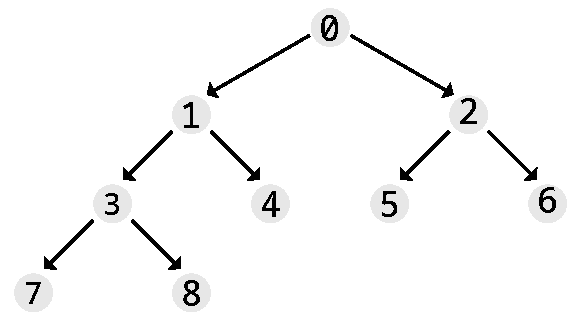
\includegraphics[scale=1]{figs/figure_heap.pdf}}
\caption{El montículo correspondiente al array que contiene los
dígitos del 0 al 8}
\label{fig.heap}
\end{figure}

Aquí presentamos una manera de construir un montículo (en 
orden alfabético parcial) desde una lista desordenada 
de letras:

\begin{verbatim}
sub construir-mont( @array, $indice is copy ) {
    my $valor-indice = @array[$indice];
    while ($indice) {
        my $padre = Int( ($indice - 1) / 2);
        my $valor-padre = @array[$padre];
        last if $valor-padre lt $valor-indice;
        @array[$indice] = $valor-padre;
        $indice = $padre;
    }
    @array[$indice] = $valor-indice;
}

sub heapify( @array ) {
    for @array.keys -> $i {
    	construir-mont @array, $i;
    }
}

my @entrada =  <m t f l s j p o b h v k n q g r i a d u e c>; 
heapify @entrada;
say @entrada;
\end{verbatim}

Nota que el montículo se construye en lugar (no hay
un necesidad para un segundo array). El array resultante
se muestra así:

\begin{verbatim}
[a b g d c k j l f h e m n q p t r o i u s v]
\end{verbatim}

¿Es este montículo correcto? Es muy difícil de saber
a primera vista y chequearlo manualmente es algo tedioso.
Al escribir un programa para construir una estructura de
datos como esta, es usualmente útil escribir algunas 
subrutinas para mostrar el contenido en un forma que 
facilite el entendimiento del resultado y el chequeo de
exactitud. El código siguiente muestras dos ejemplos
de tales subrutinas:

\begin{verbatim}
sub imprimir-mont( @array ) {
    my $inicio = 0;
    my $final = 0;
    my $último = @array.end;
    my $paso = 1;
    
    loop {
        say @array[$inicio..$final];
        last if $final == $último;
        $inicio += $paso;
        $paso *= 2;
        $final += $paso;
        $final = $último if $final > $último;
    } 
}

sub imprimir-mont2( @array ) {
    my $paso = 0;
	for @array.keys -> $actual {
	    my $h_izquierdo = @array[2 * $actual + 1];
        say "$actual\tNodo = @array[$actual];\tNo hijos" 
            and next unless defined $h_izquierdo;
        my $h_derecho = @array[2 * $actual + 2] // "' '";

        say "$actual\tNodo = @array[$actual];\tHijos: " ~ 
            " $h_izquierdo y $h_derecho";
        $paso++;
    }
}

\end{verbatim}

La primera subrutina muestra el árbol relacionado
nivel por nivel:

\begin{verbatim}
(a)
(b g)
(d c k j)
(l f h e m n q p)
(t r o i u s v)
\end{verbatim}

lo cual hace fácil dibujar el árbol (ver Figura~\ref{fig.heap2}).

\begin{figure}
\centerline
{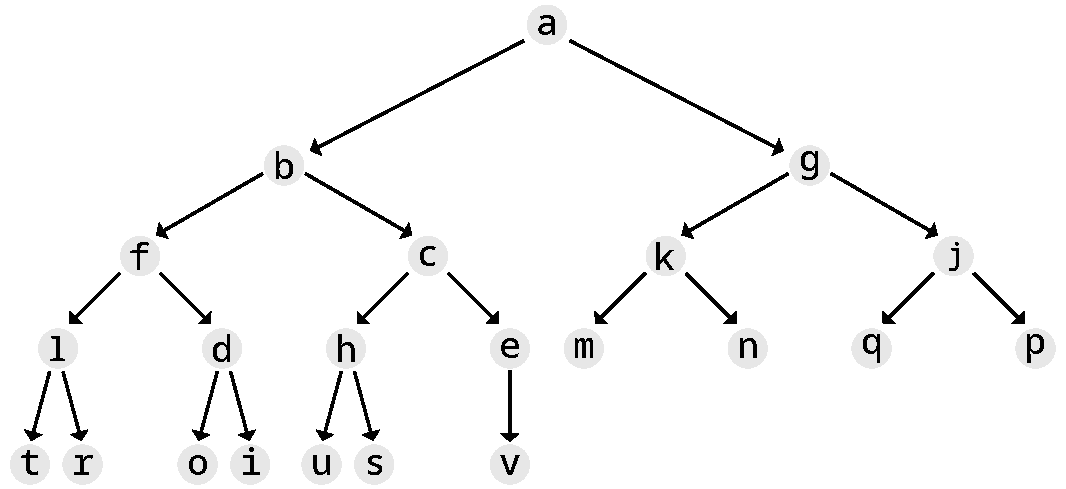
\includegraphics[scale=0.8]{figs/figure_heap2.pdf}}
\caption{El montículo correspondiente al array de letras}
\label{fig.heap2}
\end{figure}


La segunda subrutina muestra los hijos de cada nodo y hace
posible chequear fácilmente que el orden alfabético parcial
se satisface (i.e., cada nodo es menor que sus hijos):

\begin{verbatim}
0	Nodo = a;	Hijos:  b y g
1	Nodo = b;	Hijos:  d y c
2	Nodo = g;	Hijos:  k y j
3	Nodo = d;	Hijos:  l y f
4	Nodo = c;	Hijos:  h y e
5	Nodo = k;	Hijos:  m y n
6	Nodo = j;	Hijos:  q y p
7	Nodo = l;	Hijos:  t y r
8	Nodo = f;	Hijos:  o y i
9	Nodo = h;	Hijos:  u y s
10       Nodo = e;	Hijos:  v y ' '
11       Nodo = m;	No hijos
12       Nodo = n;	No hijos
(...)
21       Nodo = v;	No hijos
\end{verbatim}



\section{Depuración de Programas}
\index{debugging}

Cuando depuras un programa, y especialmente si estás 
trabajando con un error bien difícil, aquí presentamos
algunas sugerencias que podrías intentar:

\begin{description}

\item[Leer] Examina tu código, léelo, y chequea que 
diga lo que quieres decir.

\item[Ejecutar] Experimenta al hacer cambios y ejecutar las
diferentes versiones. Usualmente si muestra la cosa correcta
en el lugar correcto en el programa, el problema se vuelve 
obvio, pero algunas veces tienes que construir andamiaje para
que esto ocurra.

\item[Ejecutar con el depurador] Un {\bf depurador} es una
utilidad que te permite ejecutar un programa paso a paso,
para que puedas así seguir la ruta de ejecución y chequear
el contenido de variables importantes a puntos cruciales en
la ejecución del programa, para configurar puntos de 
interrupción, etc. Perl~6 provee un depurador, llamado 
{\tt perl6-debug}, que hace todas estas cosas posible.
Con la venida de lenguajes modernos de alto nivel, muchas
personas se resisten al uso de un depurador. Esto es un
error grave. Un depurador no te ayudará a solucionar cada 
tipo de problema, pero puede ser una utilidad inmensamente
útil. Ver la Sección~\ref{perl-debugger} para información 
adicional acerca del depurador de Perl.
\index{debugger}

\item[Reflexionar] ¡Toma tiempo para pensar! ¿Qúe tipo de error
es? ¿Sintáctico? ¿Al tiempo de ejecución? ¿Semántico?
¿Qué información puedes obtener de los mensajes de error, o desde
la salida del programa? ¿Qué tipo de error podría causar el problema
que estás observando? ¿Cuál fue el último cambio que hiciste, antes
que el problema apareciera?

\item[Depurar con el patito de goma] Si explicas el programa 
a alguien más, algunas veces encuentras la solución antes
de finalizar con la pregunta. Muy a menudo ni siquiera
necesitas la otra persona; podrías conversar con un patito
de goma. Ese es el origen de la muy conocida estrategia
conocida como la {\bf depuración del patito de goma}. 
¡Y no estoy bromeando! Lee sobre la estrategia aquí
\url{https://es.wikipedia.org/wiki/M%C3%A9todo_de_depuraci%C3%B3n_del_patito_de_goma}.
\index{rubber duck debugging}

\item[Retroceder] Algunas veces, lo mejor que puedes hacer es
retroceder, deshacer los cambios recientes, hasta que puedas
obtener un programa que funciona y que entiendas. Después puedes
comenzar la reconstrucción.

\end{description}

Los programadores principiantes algunas veces se atascan en una de
estas actividades y se olvidan de las otras. Cada actividad viene
con su propio modo de fallo.
\index{typographical error}

Por ejemplo, leer tu programa podría ayudarte si el problema es
un error tipográfico, pero no si el problema es un malentendido 
conceptual. Si no entiendes lo que tu programa hace, puedes leerlo
más 100 veces y nunca verás el error, porque el problema se encuentras en
tu cabeza.
\index{experimental debugging}


Desarrollar experimentos puede ayudarte, especialmente si ejecutas
pruebas pequeñas y simples. Pero si desarrollas experimento sin pensar 
o leer tu código, puedes caer en un patrón que llamamos ``programación de 
paso aleatorio'', el cual es el proceso de hacer cambios aleatorios hasta
que el programa haga lo correcto. Obviamente, la programación de paso aleatorio
puede tomar mucho tiempo.
\index{random walk programming}
\index{development plan!random walk programming}

Debes tomar tiempo para pensar. La depuración es como un experimento científico.
Podrías tener por lo menos una hipótesis sobre el problema (por ejemplo, 
?`cuál es el problema?). Si hay más de dos posibilidades, intenta pensar
acerca de una prueba que eliminaría uno de ellos.

Aún así, la mejores técnicas de depuración fallarán si hay muchos errores,
o si el código que estás intentando arreglar es demasiado grande y 
complicado. Algunas veces la mejor opción es retroceder, simplificar el
programa hasta que obtengas algo que funcione y que entiendas.

Los programadores principiantes son usualmente reacios a retroceder
porque no pueden tolerar el hecho de borrar una línea de código 
(aún si es algo erróneo). Si te hace sentir mejor, haz una copia de
tu programa en otro archivo antes de hacer cambios. De esa manera
puedes copiar las piezas una a la vez con cada progreso.

Encontrar un error difícil requiere leer, ejecutar (sin o con 
un depurador), reflexionar, y algunas veces retroceder. Si te atasca
en una de estas actividades, prueba las otras. 


\section{Glosario}


\begin{description}

\item[Determinista] Perteneciente a un programa que hace la misma
cosa cada vez que se ejecuta, dado la misma entrada.
\index{deterministic}

\item[Pseudoaleatorio] Perteneciente a una secuencia de números que
aparece ser aleatoria, pero es generada por un programa determinista.
\index{pseudorandom}

\item[Valor por defecto] El valor dado a un parámetro opcional si 
no se provee un argumento.
\index{default value}

\item[Sobrescribir] Reemplazar un valor por defecto con un argumento.
\index{override}

\item[Benchmarking] El proceso de elegir entre varias estructuras de datos
y algoritmos al implementar alternativas y someterlas a pruebas (
especialmente sus tiempos de duración) con una muestra de las entradas
posibles
\index{benchmarking}

\item[Depurador] Un programa que permite ejecutar un programa línea
por línea y chequea su estado a cualquier paso durante su ejecución.
\index{debugger}

\item[Depuración del patito de goma] Depuración que involucra 
explicar tu problema a un objeto inanimado tal como un patito de goma.
Articular el problema puede ayudarte a solucionarlo, aún si el patito
de goma no sabe Perl.
\index{rubber duck debugging}
\index{debugging!rubber duck}

\end{description}

\section{Ejercicio: Codificación Huffman}
\label{huffman_exercise}

La codificación Huffman es una técnica usada para la compresión de
datos, i.e., para reducir el tamaño de una pieza de datos (tal
como, por ejemplo, comprimir un archivo).

\subsection{Código de Longitud Variable}
\index{variable-length code}

Si eres familiar con el código morse, ya sabes que es un sistema
para codificar las letras del alfabeto en una serie de puntos
y rayas. Por ejemplo, la famosa señal {\tt ...---...} representa
las letras SOS, la cual constituye una llamada de ayuda reconocida
internacionalmente. La tabla en la Figura~\ref{fig.morse} 
muestra el resto de los códigos.
\index{Morse code}

\begin{figure}
\centerline
{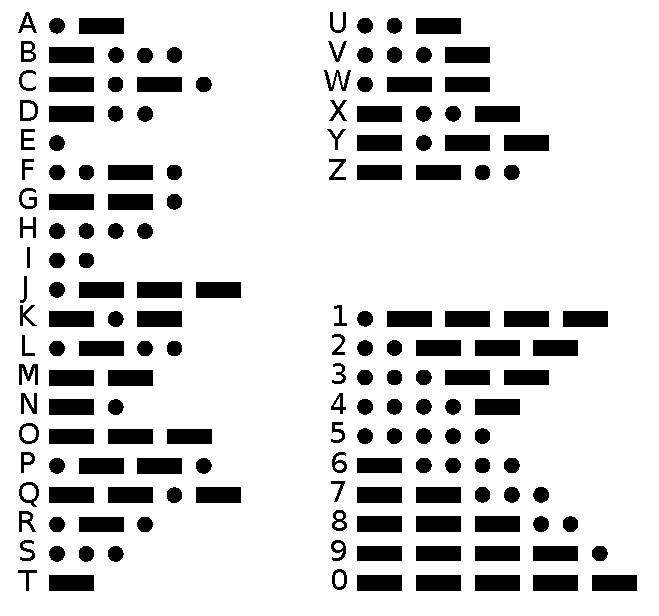
\includegraphics[scale=0.6]{figs/International_Morse_Code.pdf}}
\caption{Código Morse Internacional (dominio público)}
\label{fig.morse}
\end{figure}

El código morse (inventado entre 1836 y 1844) fue uno de los
primeros atentos de la codificación digital del alfabeto de 
un texto sencillo. El único otro atento conocido es el 
alfabeto braille (1824-1837).
\index{Morse, Samuel}
\index{braille alphabet}

Nota que algunos de los códigos son más largos que otros. Por
diseño, las letras más comunes poseen códigos más cortos. Dado
que hay un número ilimitado de códigos cortos, eso significa que
las letras y símbolos menos comunes poseen códigos más largos.
Un mensaje típico tendrás más códigos cortos que largos, lo cual
minimiza la el tiempo promedio de transmisión por letra.

Este tipo de código se conoce como códigos de longitud variable. 
En este ejercicio, estudiaremos un algoritmo para generar código
de longitud variable llamado codificación Huffman. Es un algoritmo
interesante en sí mismo, pero también hace de un ejercicio interesante
porque su implementación usa una variedad de estructuras de datos.
\index{Huffman!code}

Aquí presentamos un esquema de lo que haremos hasta al final de este capítulo:

\begin{enumerate}

\item Primeramente, usaremos una muestra de texto en inglés para generar
un tabla de los caracteres y sus frecuencias.

\item Después usaremos esta tabla de frecuencia para generar una tabla
de código.

\item Finalmente, codificaremos un mensaje con esta tabla de código y 
consiguientemente lo decodificaremos.

\end{enumerate}

\subsection{La Tabla de Frecuencias}
\index{frequency!table}

Dado que la meta es proveer las letras comunes con códigos
cortos, necesitamos saber la frecuencia con la cual cada letra
ocurre. En la historia ``The Gold Bug``\footnote{El Escarabajo de Oro} 
de Edgar Allan Poe, uno de los personajes, William~Legrand, 
usa la frecuencia de las letras para descifrar un criptograma. Él explica: 
\index{Poe, Edgar Allan}
\index{The Gold-Bug (Edgar Allan Poe)}
\index{cypher}

\begin{quote}
``Now, in English, the letter which most frequently occurs 
is e. Afterwards, the succession runs thus: a o i d h n r s 
t u y c f g l m w b k p q x z. E however predominates so 
remarkably that an individual sentence of any length is 
rarely seen, in which it is not the prevailing character.''
\footnote{
``
Ahora bien: la letra que se encuentra con mayor frecuencia en inglés es la 
e. Después, la serie es la  siguiente: a o y d h n r s t u y c f g l m w b k p q x z. 
La e predomina de un modo tan notable, que es raro encontrar una frase sola de
cierta longitud de la que no sea el carácter principal.``}
\end{quote}

Nuestra misión es chequear si Poe estaba en lo cierto. Para chequearlo,
usaremos una muestra del texto del ``The Gold Bug``, el cual
puede descargarse desde le Proyecto Gutenberg
(\url{http://www.gutenberg.org/files/2147/2147-0.txt}) 
y una variedad de otros sitios web.
\index{Project Gutenberg}

\begin{exercise}
\label{letter_frequency}
Escribe un programa que cuenta el número de veces que cada letra 
aparece en una muestra de texto. Descarga el texto de ``The Gold Bug'' 
y analiza la frecuencia de las letras.

Solución: ver Sección~\ref{sol_letter_frequency}
\end{exercise}

\subsection{Construyendo el Código Huffman}
\index{Huffman!code}

Para nuestro propósito, el código morse tiene un defecto: 
no solamente usa dos símbolos como podrías pensar, sino
que actualmente usa tres: además de los puntos y las rayas,
también usa el espacio entre los dos símbolos implícitamente,
como también espacios más largos entre dos letras.
\index{Morse code}

La razón por la cual algunos espacios son necesarios es muy simple.
Usa la tabla de código morse anterior y supón que recibes 
tres puntos (\verb'...'). Esto podría ser interpretado como la letra
``e`` tres veces, o como ``ie`` o ``ei`` o como ``s``, o como el
inicio de ``h``, ``v``, ``3``, ``4``, o ``5``. Los espacios agregados 
hacen posible distinguir entre las varias posibilidades. Pero
también hacen la transmisión de código mucho más lenta.

En 1951, David A. Huffman inventó una técnica de construcción de código
que evita este problema: provisto que sepas donde una letra dada 
comienza, no existe ninguna ambigüedad. Por ejemplo, trabajaremos 
más tarde con un código Huffman para un subconjunto pequeño
del alfabeto que luce así:
\index{Huffman, David A.}
\index{Huffman!code}

\begin{verbatim}
a => ..
e => .-
s => -.-
n => -..
t => --.
d => ---.
r => ----
\end{verbatim}

Si comienzas a leer una secuencia de puntos y rayas que representan
un texto válido compuesto con estas sietes letras, siempre puedes
decodificarlo sin ninguna ambigüedad. Si el primer símbolo es 
un punto, entonces la letra es una ``a`` o un ``e`` dependiendo 
en el símbolo siguiente. Si el primer símbolo es una raya y 
el siguiente es un punto, entonces la letra deber ser una ``s`` o
una ``n`` dependiendo del tercer símbolo. Si los primeros símbolos
son rayas, puedes similarmente determinar que la letra actual es una
``t`` (si el tercer símbolo es un punto), o una ``d`` o una ``r``. 
la cual puedes encontrar al revisar el cuarto símbolo. En resumen, 
no necesitas espacios entre los símbolos, siempre es posible
decodificar una letra sin ambigüedad.

¿Cómo podemos construir un código Huffman? Hagámoslo manualmente con
un alfabeto bien simple: las cuatros letras de las bases nitrogenadas
del ADN: A, C, T y G. Supón que queremos codificar la siguiente
cadena de texto de entrada:
\index{DNA (deoxyribonucleic acid)}
\index{alphabet}

\begin{verbatim}
CCTATCCTCGACTCCAGTCCA
\end{verbatim}

Esto resulta en la tabla de frecuencia siguiente:
\index{frequency!table}

\begin{verbatim}
C :     10      47.62
T :     5       23.81
A :     4       19.05
G :     2        9.52
\end{verbatim}

Para construir el código Huffman, comenzamos con las dos letras
menos frecuentes y las mezclamos en un símbolo nuevo temporario, 
\verb|[GA]|, el cual pretendemos es una letra compuesta nueva con una
frecuencia  de 6. En este punto, decidimos que, entre dos letras,
a la menos frecuente se le adjuntará un punto y a la otra se le
adjuntará una raya (este es una decisión arbitraria, podría
hacerse de la manera inversa). Así que decimos que el símbolo 
para la letra menos común de las dos letras (``G``) será \verb|[GA].|
y \verb|[GA]-| será el símbolo para la ``A``. 

Ahora tenemos tres letras, C, T, and [GA]. Mezclamos las dos letras
menos frecuente, ``T'' y ``[GA],'' y podemos ahora decir que el
símbolo para la ``T'' será \verb|[TGA].| y el símbolo para \verb|[GA]|
será \verb|[TGA]-|. Ahora tenemos solo dos letras restantes, 
``C'' and ``TGA``, con ``C'' siendo la menos frecuente; así que 
``C'' será un punto y ``TGA`` será una raya.

We can now unroll our dummy letters: ``T'' es \verb|[TGA].|, 
así que, reemplazando \verb|[TGA]| con su símbolo, i.e., una raya,
el código final para ``T`` será \verb|-.|; similarmente, \verb|[GA].|
ahora puede traducirse como \verb|--|. Por el mismo proceso de
sustitución, podemos ahora determinar que ``A`` es \verb|---| y ``G``
es \verb|--.|. Así que nuestra tabla final de código Huffman:
\index{Huffman!table}

\begin{verbatim}
C => .
T => -.
G => --.
A => ---
\end{verbatim}

Nota que, debido a la construcción, la letra más frecuente (C)
tiene el código más corto mientras que las letras menos
comunes (G y A) tienen los códigos más largos.

La codificación manual de cadena de texto de entrada 
\verb|CCTATCCTCGACTCCAGTCCA| con este código rinde el 
código pseudo-Morse siguiente:
\index{pseudo-Morse}

\begin{verbatim}
..-.----...-..--.---.-...-----.-...---
\end{verbatim}

Nota que nuestro código Huffman no tiene ambigüedad:
el primer punto puede solo ser una ``C``, y el segundo también.
El símbolo siguiente es una raya, que puede ser el inicio de 
las otras tres letras, pero solo la	 ``T`` puede tener un punto 
posterior. La secuencia siguiente de símbolos tiene cuatro 
rayas; esto puede solamente tres rayas de una ``A``, con la 
última raya siendo el inicio de la letra siguiente; y \verb|-.|
solo puede ser una ``T``, etc.
\index{Huffman!code}

En una codificación de Huffman real para la compresión de
archivos de texto, no usaríamos puntos y rayas, pero los 
bits 0 y 1; sin embargo, los punto y las rayas son solo
otra manera conveniente de representar esos valores
binarios. Por lo tanto, pretendamos que los puntos y las
rayas son realmente los números binarios 0 y 1.
\index{binary number}
\index{bit}

\index{data compression}
¿Realmente logramos la compresión de datos? Nuestra cadena
de pseudo-Morse tiene 38~símbolos binarios. La cadena de 
texto de entrada original tenía 21 caracteres o bytes, eso 
son 168~bits. Los datos han sido comprimidos por un factor
de 4.4. 
\index{byte}

¿Es la codificación de Huffman mejor que la codificación de 
longitud fija? Una representación de una cadena de texto donde
cada letra sería representada por dos bits (dos bits pueden
representar cuatros letras) requiere 42~símbolos. Por lo tanto,
sí, obtuvimos una mejor compresión de datos que una codificación
de longitud fija (alrededor de 10\%). Este puede parecer un logro
minúsculo, pero es actualmente un gran logro con un alfabeto tan
pequeño. Con datos textuales actuales, la codificación de Huffman
puede lograr una significante compresión de datos.


\begin{exercise}
\label{huffman_code_2}
\begin{enumerate}

\item Escribe un programa que realiza codificación de Huffman
de una cadena de texto de caracteres simple. Puedes comenzar con
el ejemplo de ADN más arriba. No te preocupes si no obtienes la
misma tabla de Huffman de más arriba: pueden haber más código
de Huffman para una cadena de texto dada; pero chequea que obtengas
un código que no sea ambiguo.
\index{Huffman!code}

\item Haz una prueba con cadenas de texto que tienen un alfabeto
más grande (probablemente querrás comenzar con un alfabeto
relativamente pequeño porque, por lo contrario,
puede ser tedioso chequear el resultado manualmente).
 
\item Escribe una subrutina que codifique una cadena de texto
de entrada en pseudo-Morse usando la tabla de Huffman generada
anteriormente.
\index{pseudo-Morse}
\index{alphabet}

\item Escribe una subrutina que decodifique la salida pseudo-Morse
que has generado para la pregunta anterior.
\end{enumerate}
%
Solución: ver Sección~\ref{sol_huffman_code_2}.
\index{Huffman!code}
\end{exercise}

